\appendix

\section{AIMSpice Code}
\label{appendix:aimspice}

\begin{lstlisting}[style=aimspiceStyle, caption=1-bit register in AIMSPICE, label=testcode]
1Bit Register

**************************************************************
* Including the file containing the NMOS and PMOS transistors
.include gpdk90nm_tt.cir
**************************************************************

**************************************************************
.PARAM W_VAL=1500n
.PARAM L_VAL=300n
**************************************************************

**************************************************************
* Subcircuit for a NOT gate 
.subckt NOT GND VDD A OUT
XMP1 OUT A VDD VDD PMOS1V W=W_VAL L=L_VAL 
XMN1 OUT A GND GND NMOS1V W=W_VAL L=L_VAL
.ends NOT
**************************************************************

**************************************************************
* Subcircuit for a NAND gate 
.subckt NAND GND VDD A B OUT
XMP1 VDD A OUT VDD PMOS1V W=W_VAL L=L_VAL 
XMP2 VDD B OUT VDD PMOS1V W=W_VAL L=L_VAL 
XMN1 OUT A C C NMOS1V W=W_VAL L=L_VAL 
XMN2 C B GND GND NMOS1V W=W_VAL L=L_VAL 
.ends NAND
**************************************************************

**************************************************************
* Subcircuit for an AND gate 
.subckt AND GND VDD A B OUT
XAND1 GND VDD A B C NAND
XNOT1 GND VDD C OUT NOT
.ends AND
**************************************************************

**************************************************************
* Subcircuit for a TRANSMISSION gate 
.subckt TRANS GND VDD IN EN_N EN_P OUT
XMN1 IN EN_N OUT GND NMOS1V W=W_VAL L=L_VAL
XMP1 IN EN_P OUT VDD PMOS1V W=W_VAL L=L_VAL 
.ends TRANS
**************************************************************

**************************************************************
* Subcircuit for a MUX for set and reset
.subckt MUX GND VDD S R DI Q DO
XNOT1 GND VDD S 1 NOT
XTRANS1 GND VDD DI S 1 2 TRANS
XTRANS2 GND VDD Q 1 S 2 TRANS
XNOT2 GND VDD R 3 NOT
XAND GND VDD 2 3 DO AND
.ends 
**************************************************************

**************************************************************
*Subcircuit for a D FLIP FLOP using TRANSMITION gates 
.subckt FLOP GND VDD CLK D Q 
XNOT1 GND VDD D 1 NOT
XNOT_CLK GND VDD CLK NOTCLK NOT
XTRANS1 GND VDD 1 NOTCLK CLK 2 TRANS
XNOT2 GND VDD 2 3 NOT
XNOT3 GND VDD 3 4 NOT 
XTRANS2 GND VDD 4 CLK NOTCLK 2 TRANS
XTRANS3 GND VDD 3 CLK NOTCLK 5 TRANS
XNOT4 GND VDD 5 6 NOT
XNOT5 GND VDD 6 7 NOT
XTRANS4 GND VDD 7 NOTCLK CLK 5 TRANS
XNOT6 GND VDD 6 Q NOT
.ends
**************************************************************

**************************************************************
* Subcircuit for 1bit register with set and reset
.subckt REGISTER GND VDD CLK S R D Q 
XMUX1 GND VDD S R D Q 1 MUX
XFLOP GND VDD CLK 1 Q FLOP
.ends
**************************************************************


**************************************************************
.PARAM RISE_TIME=0.5n 
.PARAM FALL_TIME=0.5n 
.PARAM CLK_PERIOD=20n 
.PARAM CLK_HIGH=10n 
.PARAM V_DD=0.85
.PARAM C_VDD=0.85


*Setting VDD = 0.85, the D, CLK, S and R as different square waves
VDD 1 0 V_DD
VD D 0 PULSE(0 C_VDD 25n RISE_TIME FALL_TIME 20ns 40ns)
VCLK CLK 0 PULSE(0 C_VDD 0 RISE_TIME FALL_TIME CLK_HIGH CLK_PERIOD)
VS S 0 PULSE(0 C_VDD 20n RISE_TIME FALL_TIME 60n 120n)
VR R 0 PULSE(0 C_VDD 145n RISE_TIME FALL_TIME 50n 100n)
**************************************************************

**************************************************************
*Defining the register
XREG 0 1 CLK S R D Q REGISTER
**************************************************************

**************************************************************
*Plotting Q, D, CLK, S and R for the register
.plot v(Q)
.plot v(D)
.plot v(CLK)
.plot v(S) 
.plot v(R)
**************************************************************
\end{lstlisting}




\section{Verilog Code}
\label{appendix:Verilog-code}

\begin{lstlisting}[style=verilogStyle, caption=Half Adder in Verilog, label=verilog_halfadder]
module Half_Adder ( A_0 ,B_0 ,S_0 ,C_0 );

input A_0 ;
wire A_0 ;
input B_0 ;
wire B_0 ;
output S_0 ;
wire S_0 ;
output C_0 ;
wire C_0 ;

and(C_0, A_0, B_0);
xor(S_0, A_0, B_0);

endmodule
\end{lstlisting}


\begin{lstlisting}[style=verilogStyle, caption=Full Adder in Verilog, label=verilog_fulladder]
module Full_Adder ( C_I ,S_O ,A_I ,C_O ,B_I );

input C_I ;
wire C_I ;
output S_O ;
wire S_O ;
input A_I ;
wire A_I ;
output C_O ;
wire C_O ;
input B_I ;
wire B_I ;

wire w1,w2,w3;
xor(w1, A_I, B_I);
and(w2, A_I, B_I); 
and(w3, w1, C_I);
xor(S_O, w1, C_I);
or(C_O, w2, w3); 

endmodule
\end{lstlisting}


\begin{lstlisting}[style=verilogStyle, caption=8-bit adder in Verilog, label=verilog_eightbitadder]
`include "Half_Adder.v"
`include "Full_Adder.v"

module eightbit_adder (
    input [7:0] A,
    input [7:0] B,
    output [7:0] S
);

wire [7:0] carry;
wire [7:0] carry_out;

Half_Adder ha_instance_0 (
    .A_0(A[0]),
    .B_0(B[0]),
    .S_0(S[0]),
    .C_0(carry[0])
);

Full_Adder FA_1 (
    .A_I(A[1]),
    .B_I(B[1]),
    .C_I(carry[0]),
    .S_O(S[1]),
    .C_O(carry_out[1])
);

Full_Adder FA_2 (
    .A_I(A[2]),
    .B_I(B[2]),
    .C_I(carry_out[1]),
    .S_O(S[2]),
    .C_O(carry_out[2])
);

Full_Adder FA_3 (
    .A_I(A[3]),
    .B_I(B[3]),
    .C_I(carry_out[2]),
    .S_O(S[3]),
    .C_O(carry_out[3])
);

Full_Adder FA_4 (
    .A_I(A[4]),
    .B_I(B[4]),
    .C_I(carry_out[3]),
    .S_O(S[4]),
    .C_O(carry_out[4])
);

Full_Adder FA_5 (
    .A_I(A[5]),
    .B_I(B[5]),
    .C_I(carry_out[4]),
    .S_O(S[5]),
    .C_O(carry_out[5])
);

Full_Adder FA_6 (
    .A_I(A[6]),
    .B_I(B[6]),
    .C_I(carry_out[5]),
    .S_O(S[6]),
    .C_O(carry_out[6])
);

Full_Adder FA_7 (
    .A_I(A[7]),
    .B_I(B[7]),
    .C_I(carry_out[6]),
    .S_O(S[7]),
    .C_O(carry_out[7])
);

endmodule
\end{lstlisting}


\begin{lstlisting}[style=verilogStyle, caption=D Flip-Flop in Verilog, label=verilog_dflipflop]
module D_Flip_Flop ( input D_flip , output Q_flip , input clk_flip );
	
	wire clk_bar_flip; 
	not(clk_bar_flip, clk_flip);
	not(w1_flip, D_flip);	  
	wire w2_flip;
	cmos(w2_flip, w1_flip, clk_bar_flip, clk_flip);	
	wire w3_flip;
	not(w3_flip, w2_flip); 
	wire w4_flip;
	not(w4_flip, w3_flip);
	cmos(w2_flip, w4_flip, clk_flip, clk_bar_flip);	 
	wire w5_flip;
	cmos(w5_flip, w3_flip, clk_flip, clk_bar_flip);
	wire w6_flip, w7_flip;
	not(w6_flip, w5_flip);
	not(w7_flip, w6_flip);
	cmos(w5_flip, w7_flip, clk_bar_flip, clk_flip);	 
	not(Q_flip, w6_flip);

endmodule
\end{lstlisting}


\begin{lstlisting}[style=verilogStyle, caption=Register control circuit in Verilog, label=verilog_regmux]
module Reg_mux (
    input S_mux,
    input R_mux,
    input D_I_mux,
    input Q_mux,
    output D_O_mux
);			  
wire Y_mux, sbar, rbar;	
not(sbar,S_mux);
not(rbar,R_mux); 

cmos(Y_mux,D_I_mux, S_mux, sbar);
cmos(Y_mux,Q_mux,sbar,S_mux);
and(D_O_mux, rbar, Y_mux);

endmodule
\end{lstlisting}


\begin{lstlisting}[style=verilogStyle, caption=One-bit register in Verilog, label=verilog_onebitregister]
`include "Reg_mux.v"
`include "D_Flip_Flop.v"

module onebit_register (input D, input S, input R, input CLK, output Q);

  wire D_O_mux; // Output from the control circuit

  Reg_mux mux_instance (
    .S_mux(S),
    .R_mux(R),
    .D_I_mux(D), 
    .Q_mux(Q), // Connect the Q output of the flip-flop to the input of the multiplexer  
    .D_O_mux(D_O_mux)
  );

  D_Flip_Flop flip_flop_instance (
    .D_flip(D_O_mux), // Connect the input of the flip-flop to the multiplexer's output
    .Q_flip(Q),
    .clk_flip(CLK)
  );

endmodule
\end{lstlisting}


\begin{lstlisting}[style=verilogStyle, caption=8-bit register, label=verilog_eightbitregister]
`include "onebit_register.v"

module eightbit_register (input s_eight , input r_eight ,input clk_eight, 
							input [7:0] d_eight ,output [7:0] q_eight );
	
	onebit_register onebit_instance0 (
	    .S(s_eight),
	    .R(r_eight),
		.CLK(clk_eight),
	    .D(d_eight[0]), // Connect the corresponding bit of d_eight to onebit_register
	    .Q(q_eight[0])
	); 
	onebit_register onebit_instance1 (
	    .S(s_eight),
	    .R(r_eight),
		.CLK(clk_eight),
	    .D(d_eight[1]), // Connect the corresponding bit of d_eight to onebit_register
	    .Q(q_eight[1])
	);
	onebit_register onebit_instance2 (
	    .S(s_eight),
	    .R(r_eight),
		.CLK(clk_eight),
	    .D(d_eight[2]), // Connect the corresponding bit of d_eight to onebit_register
	    .Q(q_eight[2])
	);		   
	onebit_register onebit_instance3 (
	    .S(s_eight),
	    .R(r_eight),
		.CLK(clk_eight),
	    .D(d_eight[3]), // Connect the corresponding bit of d_eight to onebit_register
	    .Q(q_eight[3])
	);
	onebit_register onebit_instance4 (
	    .S(s_eight),
	    .R(r_eight),
		.CLK(clk_eight),
	    .D(d_eight[4]), // Connect the corresponding bit of d_eight to onebit_register
	    .Q(q_eight[4])
	);
	onebit_register onebit_instance5 (
	    .S(s_eight),
	    .R(r_eight),
		.CLK(clk_eight),
	    .D(d_eight[5]), // Connect the corresponding bit of d_eight to onebit_register
	    .Q(q_eight[5])
	);
	onebit_register onebit_instance6 (
	    .S(s_eight),
	    .R(r_eight),
		.CLK(clk_eight),
	    .D(d_eight[6]), // Connect the corresponding bit of d_eight to onebit_register
	    .Q(q_eight[6])
	);
	onebit_register onebit_instance7 (
	    .S(s_eight),
	    .R(r_eight),
		.CLK(clk_eight),
	    .D(d_eight[7]), // Connect the corresponding bit of d_eight to onebit_register
	    .Q(q_eight[7])
	);

endmodule
\end{lstlisting}


\begin{lstlisting}[style=verilogStyle, caption=MAC in Verilog, label=verilog_MAC]
`include "twobit_multiplier.v"
`include "eightbit_adder.v"
`include "eightbit_register.v"

module MAC(
    input [1:0] A, 
    input [1:0] B, 
    input CLK, 
    input [1:0] CTRL, 
    output [7:0] Y
    );

    wire [1:0] A, B, CTRL;
    wire CLK;
    wire [7:0] Y;
    wire [3:0] PROD;
    wire [7:0] SUM;


    twobit_multiplier multiplier_instance(.A(A), .B(B), .O(PROD));
    eightbit_adder adder_instance(.A({4'b0000, PROD}), .B(Y), .S(SUM));
    eightbit_register register_instance(
        .s_eight(CTRL[0]), 
        .r_eight(CTRL[1]), 
        .clk_eight(CLK),
        .d_eight(SUM),
        .q_eight(Y));
    
endmodule
\end{lstlisting}


\begin{lstlisting}[style=verilogStyle, caption=FSM in Verilog, label=verilog_FSM]
`include "onebit_register.v"

module Mealy_FSM(
    input RunIN, 
    input ResetIN, 
    input CLK, 
    output RunOUT, 
    output ResetOUT
    );

    //Define wires

    wire RunIN, ResetIN, CLK, RunOUT, ResetOUT, Set, A, B;
    wire [1:0] C, N;

    //The FSM should always take in the next state

    assign Set = 1;

    //Define the registers

    onebit_register Reg0(.D(N[0]), .S(Set), .R(ResetIN), .CLK(CLK), .Q(C[0]));
    onebit_register Reg1(.D(N[1]), .S(Set), .R(ResetIN), .CLK(CLK), .Q(C[1]));

    //Throughput the reset-signal

    assign ResetOUT = ResetIN;

    //Define logic gates and MUX

    xor(N[0], C[0], RunIN);
    and(A, C[0], RunIN);
    xor(N[1], A, C[1]);
    nand(B, C[0], C[1]);
    and(RunOUT, B, RunIN);

endmodule
\end{lstlisting}


\begin{lstlisting}[style=verilogStyle, caption=Full MAC circuit in Verilog, label=verilog_fullmac]
`include "Mealy_FSM.v"
`include "MAC.v"

module MAC_FULL(
    input [1:0] I, 
    input [1:0] A, 
    input [1:0] B, 
    input CLK, 
    output [7:0] Y
    );

    wire CLK;
    wire [1:0] I, CTRL, A, B;
    wire [7:0] Y;

    Mealy_FSM fsm_instance(
        .RunIN(I[0]), 
        .ResetIN(I[1]), 
        .CLK(CLK), 
        .RunOUT(CTRL[0]), 
        .ResetOUT(CTRL[1])
    );
        
    MAC mac_instance(
        .A(A),
        .B(B),
        .CLK(CLK),
        .CTRL(CTRL),
        .Y(Y)
    );

endmodule
\end{lstlisting}

\section{Verilog Testbenches}
\label{sec:verilog_testbenches}

\begin{lstlisting}[style=verilogStyle, caption=Multiplier Testbench in Verilog, label=verilog_multiplierTB]
`timescale 1 ns / 1 ps
`include "twobit_multiplier.v"

module Multiplier_Testbench();
    reg [1:0] A, B;
    wire [3:0] O;
    integer errors;
    integer Acount, Bcount;

    twobit_multiplier mul_instance (.A(A), .B(B), .O(O));
    initial begin
        $dumpfile("Multiplier_Testbench.vcd");
        $dumpvars(0, Multiplier_Testbench);
        errors = 0;

        for(Acount = 0 ; Acount < 4 ; Acount++) begin
            for(Bcount = 0 ; Bcount < 4 ; Bcount++) begin
                A = Acount;
                B = Bcount;
                #1;
                if((A*B) != O) begin
                    $display("Error: ",A,"*",B,"=",O);
                    errors++;
                end else begin
                    $display(A,"*",B,"=",O);
                end
            end
        end
        if(errors==0)begin
            $display("No errors found");
        end else begin
            $display(errors," errors found. Reevaluate design.");
        end
        $finish;
    end

endmodule
\end{lstlisting}


\begin{lstlisting}[style=verilogStyle, caption=Adder Testbench in Verilog, label=verilog_adderTB]
`timescale 1 ns / 1 ps
`include "eightbit_adder.v"

module Adder_Testbench();
    reg [7:0] A, B;
    wire [7:0] S;
    integer errors;
    integer Acount, Bcount;

    eightbit_adder adder_instance(.A(A), .B(B), .S(S));

    initial begin
        $dumpfile("Adder_Testbench.vcd");
        $dumpvars(0, Adder_Testbench);
        errors = 0;
        for(Acount = 0 ; Acount < 256 ; Acount++) begin
            for(Bcount = 0 ; Bcount < 256 ; Bcount++) begin
                A = Acount;
                B = Bcount;
                #1;
                if((A+B) == S) begin
                    $display(A,"+",B,"=",S);
                end else begin
                    $display("Error: ", A, "+", B, "=",S);
                    errors++;
                end
            end
        end
        if(errors==0)begin
            $display("Congratulations! No errors found.");
        end else begin
            $display("WARNING! ",errors," errors found. Reevaluate circuit.");
        end
        $finish;
    end
endmodule
\end{lstlisting}


\begin{lstlisting}[style=verilogStyle, caption=Register Testbench in Verilog, label=verilog_registerTB]
`timescale 1 ns / 1 ps
`include "eightbit_register.v"

module Register_Testbench();
    parameter CLK_PERIOD = 10;
    reg s_eight,r_eight,clk_eight;
    reg [7:0] d_eight;
    wire [7:0] q_eight;
    integer errors;
    integer temp;

    eightbit_register register_instance(
        .s_eight(s_eight), 
        .r_eight(r_eight),
        .clk_eight(clk_eight),
        .d_eight(d_eight),
        .q_eight(q_eight)
    );

    always #((CLK_PERIOD / 2)) clk_eight = ~clk_eight;

    initial begin
        $dumpfile("Register_Testbench.vcd");
        $dumpvars(0, Register_Testbench);
        errors = 0;
        clk_eight = 0;

        //Setting a value in the register and checking output
        s_eight = 1;
        r_eight = 0;
        d_eight = 123;
        #CLK_PERIOD;

        //Testing controlsignals 00 for all inputs d
        s_eight = 0;
        r_eight = 0;
        for(temp = 0 ; temp < 256 ; temp++) begin
            d_eight = temp;
            #CLK_PERIOD;
            if(q_eight != 123) begin
                $display("Error: Value overwritten when S=0");
                errors++;
            end
        end

        //Testing controllsignals 01 and 11 for all inputs d
        s_eight = 0;
        r_eight = 1;
        for(temp = 0 ; temp < 256 ; temp++) begin
            d_eight = temp;
            #CLK_PERIOD;
            if(q_eight != 0) begin
                $display("Error: Output not zero when R=1");
                errors++;
            end
        end

        s_eight = 1;
        r_eight = 1;
        for(temp = 0 ; temp < 256 ; temp++) begin
            d_eight = temp;
            #CLK_PERIOD;
            if(q_eight != 0) begin
                $display("Error: Output not zero when R=1");
                errors++;
            end
        end

        //Testing all inputs d with control signals 10
        s_eight = 1;
        r_eight = 0;
        for(temp = 0 ; temp < 256 ; temp++) begin
            d_eight = temp;
            #CLK_PERIOD;
            if(q_eight != d_eight) begin
                $display("Error: Value not set when S=1");
                errors++;
            end
        end
        if(errors==0) begin
            $display("Congratulations! No errors found.");
        end else begin
            $display("WARNING! ",errors, " errors found. Reevaluate circuit.");
        end
        $finish;
    end
endmodule
\end{lstlisting}


\begin{lstlisting}[style=verilogStyle, caption=FSM Testbench in Verilog, label=verilog_FSMTB]
`timescale 1 ns / 1 ps
`include "Mealy_FSM.v"

module Testbench;

    reg CLK;
    reg [1:0] I;
    wire [1:0] O;

    always #5 CLK = ~CLK;

    Mealy_FSM uut(
        .RunIN(I[0]), 
        .ResetIN(I[1]), 
        .CLK(CLK), 
        .RunOUT(O[0]), 
        .ResetOUT(O[1]));

    initial begin

        $dumpfile("TB_dumpfile.vcd");
        $dumpvars(0, Testbench);

        CLK = 0;
        I = 3;
        #10;
        I = 1;
        #50;
        for(integer temp = 0 ; temp < 5 ; temp++)begin
            I = $random % 4;
            #40;
        end
        $finish;
    end

endmodule
\end{lstlisting}

\begin{lstlisting}[style=verilogStyle, caption=Full MAC Testbench in Verilog, label=verilog_FULLMAC_TB]
`timescale 1 ns / 1 ps
`include "MAC_FULL.v"

module TB;

    integer randomSeed = 5;
    reg [1:0] I, A, B;
    reg CLK;
    wire [7:0] Y;

    MAC_FULL uut(.*);

    always #5 CLK = ~CLK;
    always #10 A = $random(randomSeed) % 4;
    always #10 B = $random % 4;

    initial begin
        $dumpfile("TB_dumpfile.vcd");
        $dumpvars(0, TB);

        CLK = 0;
        I = 3;
        A = $random % 4;
        B = $random % 4;
        #10;
        I = 1;
        #100;
        I=0;
        #60;
        I = 3;
        #10;
        I = 1;
        #150;
        $finish;
    end

endmodule
\end{lstlisting}


\section{Optional (rename based on what you put here)}
Sometimes one might end up running a lot of simulations, and then find out that not all of them were relevant enough to present in the actual report. Additional figures and results can then be included here (with a brief explanation so that the reader knows what they are looking at). This section of the appendix is optional, and might not be relevant for your group. 

Anything added here will not affect the grade directly, but might contribute to the overall impression of the work you have done (which is part of what we grade). Your grade will NOT be affected negatively if only the AIMSpice and Verilog code is in the appendix.

\newpage
\section{AimSpice Plots}
\label{appendix:aimspicePlots}

\begin{figure}[H]
    \begin{minipage}{0.5\textwidth}
        \centering
        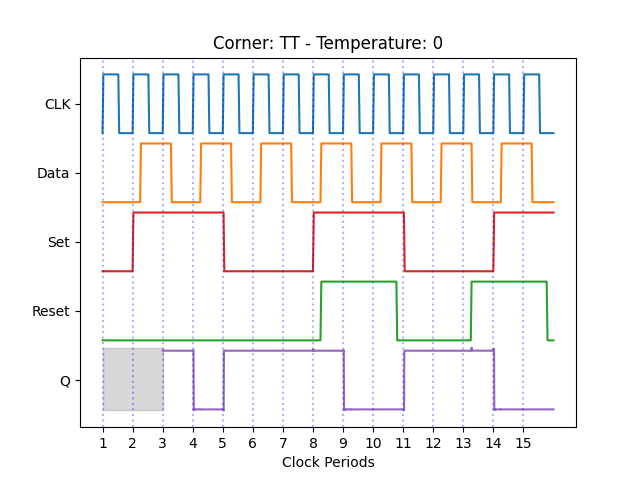
\includegraphics[width=\textwidth]{Figures/Aimspice_Plots/TT_0.png}
        \caption{Plot of register for TT corner}
        \label{fig:TT0}
    \end{minipage}%
    \begin{minipage}{0.5\textwidth}
        \centering
        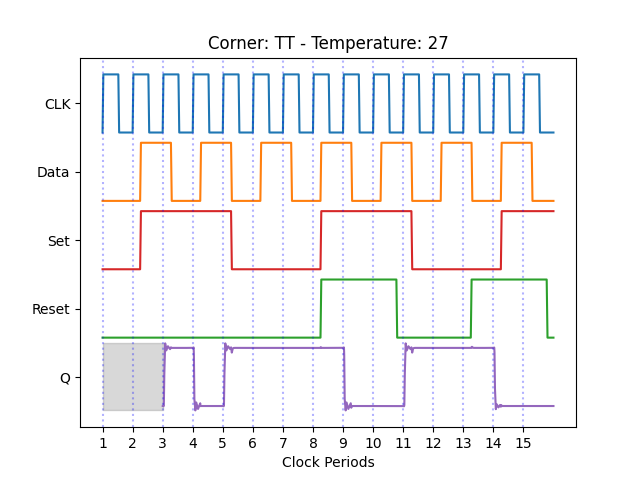
\includegraphics[width=\textwidth]{Figures/Aimspice_Plots/TT_27.png}
        \caption{Plot of register for TT corner}
        \label{fig:TT27}
    \end{minipage}
\end{figure}
\begin{figure}[H]
    \centering
    \begin{minipage}{0.5\textwidth}
        \centering
        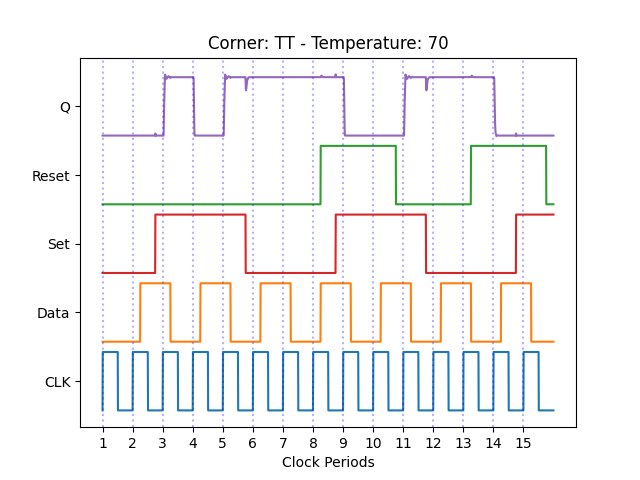
\includegraphics[width=\textwidth]{Figures/Aimspice_Plots/TT_70.png}
        \caption{Plot of register for TT corner}
        \label{fig:TT70}
    \end{minipage}%
\end{figure}

\begin{figure}[H]
    \begin{minipage}{0.5\textwidth}
        \centering
        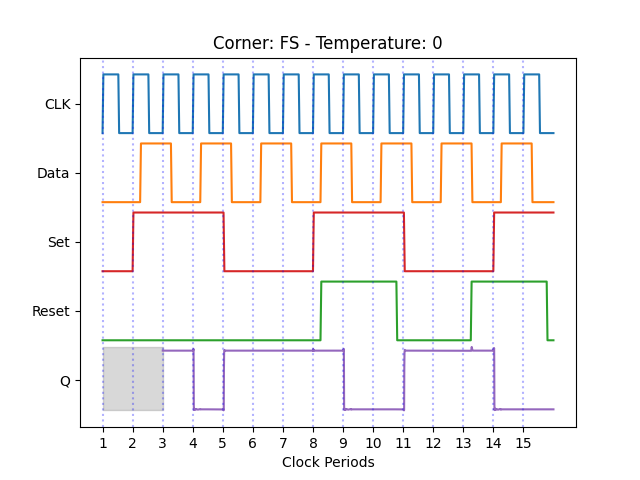
\includegraphics[width=\textwidth]{Figures/Aimspice_Plots/FS_0.png}
        \caption{Plot of register for FS corner}
        \label{fig:FS0}
    \end{minipage}%
    \begin{minipage}{0.5\textwidth}
        \centering
        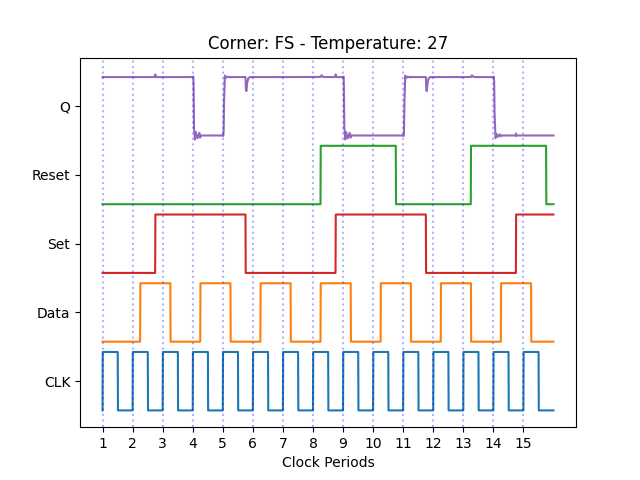
\includegraphics[width=\textwidth]{Figures/Aimspice_Plots/FS_27.png}
        \caption{Plot of register for FS corner}
        \label{fig:FS27}
    \end{minipage}
\end{figure}
\begin{figure}[H]
    \centering
    \begin{minipage}{0.5\textwidth}
        \centering
        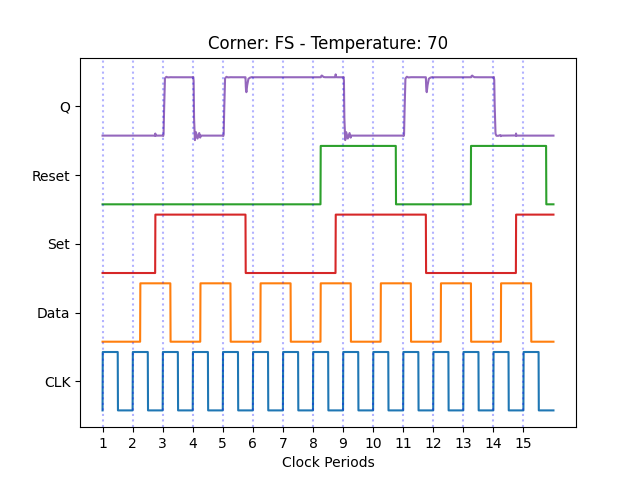
\includegraphics[width=\textwidth]{Figures/Aimspice_Plots/FS_70.png}
        \caption{Plot of register for FS corner}
        \label{figFS70}
    \end{minipage}%
\end{figure}

\begin{figure}[H]
    \begin{minipage}{0.5\textwidth}
        \centering
        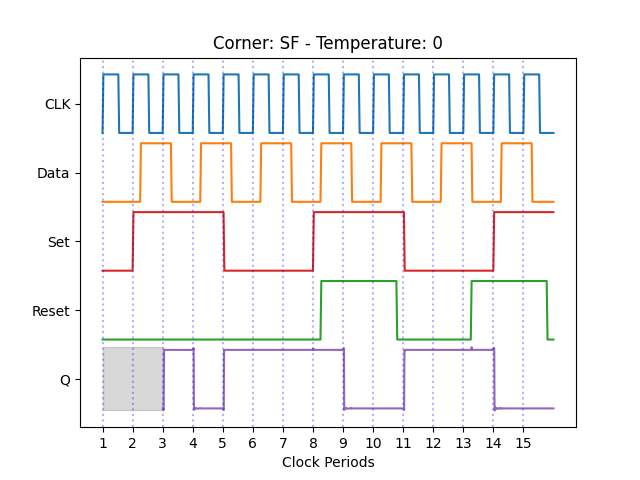
\includegraphics[width=\textwidth]{Figures/Aimspice_Plots/SF_0.png}
        \caption{Plot of register for SF corner}
        \label{fig:SF0}
    \end{minipage}%
    \begin{minipage}{0.5\textwidth}
        \centering
        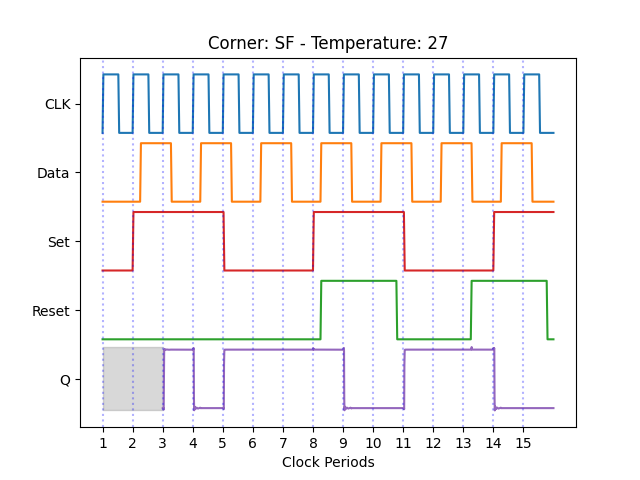
\includegraphics[width=\textwidth]{Figures/Aimspice_Plots/SF_27.png}
        \caption{Plot of register for SF corner}
        \label{fig:SF27}
    \end{minipage}
\end{figure}
\begin{figure}[H]
    \centering
    \begin{minipage}{0.5\textwidth}
        \centering
        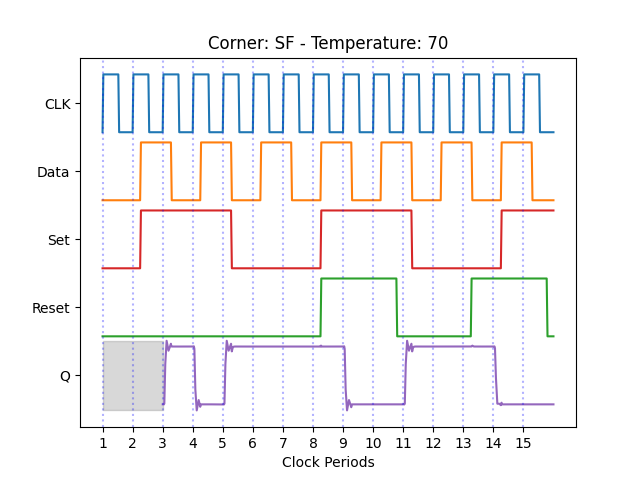
\includegraphics[width=\textwidth]{Figures/Aimspice_Plots/SF_70.png}
        \caption{Plot of register for SF corner}
        \label{fig:SF70}
    \end{minipage}%
\end{figure}

\begin{figure}[H]
    \begin{minipage}{0.5\textwidth}
        \centering
        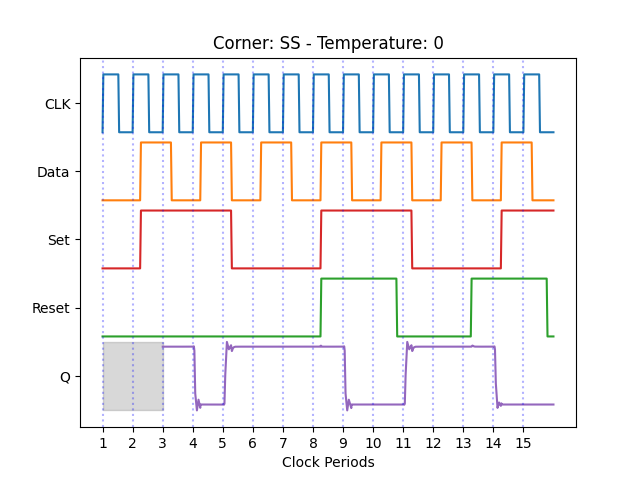
\includegraphics[width=\textwidth]{Figures/Aimspice_Plots/SS_0.png}
        \caption{Plot of register for SS corner}
        \label{fig:SS0}
    \end{minipage}%
    \begin{minipage}{0.5\textwidth}
        \centering
        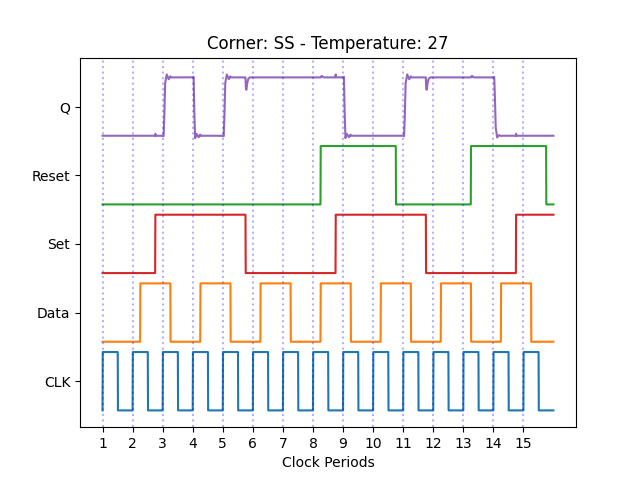
\includegraphics[width=\textwidth]{Figures/Aimspice_Plots/SS_27.png}
        \caption{Plot of register for SS corner}
        \label{fig:SS27}
    \end{minipage}
\end{figure}
\begin{figure}[H]
    \centering
    \begin{minipage}{0.5\textwidth}
        \centering
        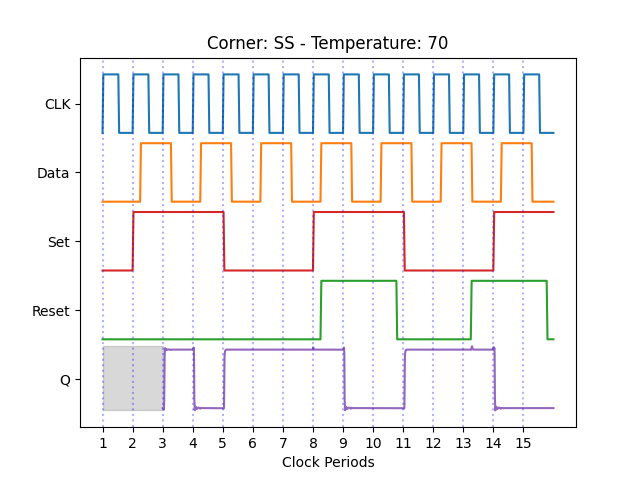
\includegraphics[width=\textwidth]{Figures/Aimspice_Plots/SS_70.png}
        \caption{Plot of register for SS corner}
        \label{fig:SS70}
    \end{minipage}%
\end{figure}

\begin{figure}[H]
    \begin{minipage}{0.5\textwidth}
        \centering
        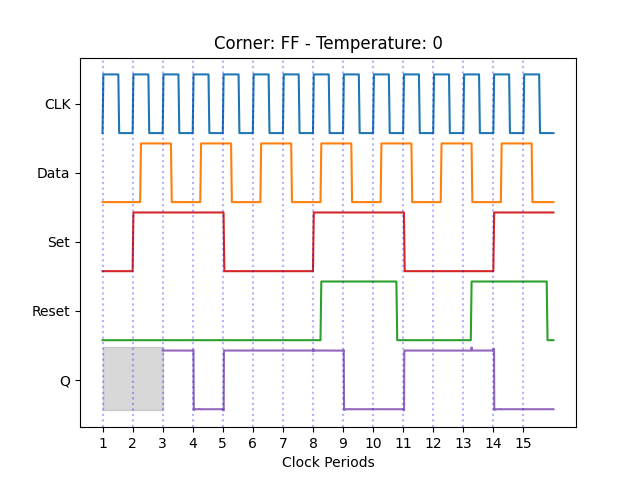
\includegraphics[width=\textwidth]{Figures/Aimspice_Plots/FF_0.png}
        \caption{Plot of register for FF corner}
        \label{fig:FF0}
    \end{minipage}%
    \begin{minipage}{0.5\textwidth}
        \centering
        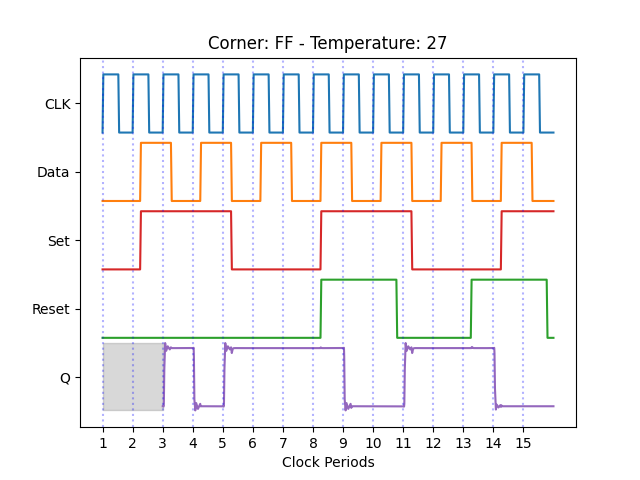
\includegraphics[width=\textwidth]{Figures/Aimspice_Plots/FF_27.png}
        \caption{Plot of register for FF corner}
        \label{fig:FF27}
    \end{minipage}
\end{figure}
\begin{figure}[H]
    \centering
    \begin{minipage}{0.5\textwidth}
        \centering
        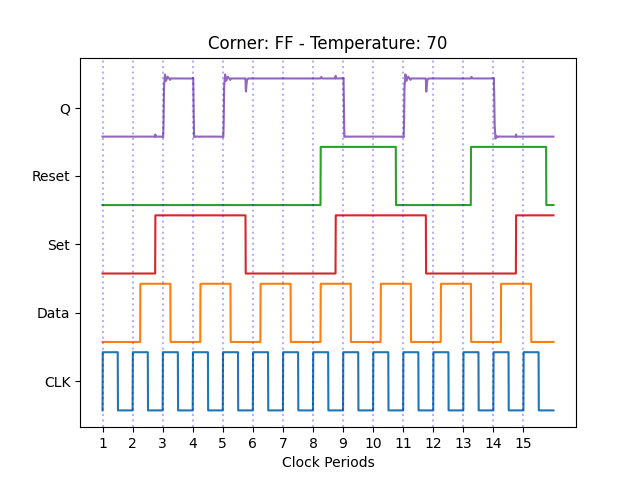
\includegraphics[width=\textwidth]{Figures/Aimspice_Plots/FF_70.png}
        \caption{Plot of register for FF corner}
        \label{fig:FF70}
    \end{minipage}%
\end{figure}
